\section{Import / Export}
\label{sectionImportExport}

Mit Hilfe dieser Implementierung werden Import- bzw. Exportprozesse bereitgestellt, die eine Schnittstelle zu zwei unterschiedlichen Endpunkten anbieten. Zum einen kann mit einer relationalen Datenbank \textbf{MySQL} und zum anderen mit der Open Office Lösung \textbf{Libre Office} und dem dazugehörigen Kalkulationsprogramm \textbf{Calc} kommuniziert werden. Es ist somit möglich, Daten aus einer Tabellensprache in einer MySQL-Datenbank zu archivieren und auszulesen. Außerdem können Daten aus einer *.ods-Datei, die das Dateiformat von Libre Office Calc darstellt, ausgelesen werden. Ferner kann aus der Tabellensprache eine *.ods-Datei generiert werden.
\\\\
In den nächsten zwei Unterkapiteln \ref{subsectionMySql} und \ref{subsectionLibreOffice} werden die wichtigsten Kernfunktionalitäten und die dafür benötigten Objekte (Models) näher erläutert. Hilfsfunktionen werden in dieser Dokumentation nur aufgelistet und kurz beschrieben.

\subsection{MySQL}
\label{subsectionMySql}
\subsubsection{Kurzbeschreibung}
\label{mysqlDescription}
Um das Ziel zu erlangen, statistische Tabellen mit Hilfe einer neuen Tabellensprache zu erzeugen, musst eine Grundlage zur Datenbeschaffung bzw. Archivierung geschaffen werden. Diese Grundlage widerspiegelt sich in einer Anbindung an eine relationale Datenbank. Der Fokus wird in diesem Projekt auf die MySQL-Datenbank gelegt.

\subsubsection{Models}
\label{mysqlModels}
\textbf{MSqlConnectionParameters}\\
Das hier generierte Model beinhaltet alle nötigen Parameter, um eine stabile Verbindung zu einer Datenbank aufzubauen. Neben der IP-Adresse des MySQL-Servers und der dazugehörige Port (Defaultwert 3306) ist zudem der Name der Datenbank, der Username eines Admins des MySQL-Servers und das dazugehörige Password von Nöten.

\begin{lstlisting}[caption=Parameter für eine MySQL-Datenbankverbindung, language=Java]
private String _ip;
private int _port;
private String _dbName;
private String _username;
private String _password;
\end{lstlisting}
\textbf{MSqlTableContent}\\
Dieses Model kapselt alle nötigen Daten einer MySQL-Datenbank in ein Objekt. Hierbei repräsentiert die Property {\_}dbName den Namen der Datenbanktabelle. In der ArrayList {\_}headlines, die auf den Datentyp "String" festgezogen ist, werden die Tabellenüberschriften abgelegt und einem festen Index zugewiesen. Dieser Index lässt sich wiederum in der ArrayList {\_}content mit dem Typ ArrayList<String> wiederfinden. Durch die Indizes lässt sich der Tabelleninhalt stets der korrekten Tabellenüberschrift zuordnen.

\begin{lstlisting}[caption=Repräsentation einer MySQL-Tabelle als Java-Objekt, language=Java]
private String _dbName;
private ArrayList<String> _headlines;
private ArrayList<ArrayList<String>> _content;
\end{lstlisting}

\subsubsection{Kernfunktionalitäten}
\label{mysqlCore}
Alle Funktionalitäten für das Arbeiten mit einer MySQL-Datenbank beinhaltet die Klasse "DatabaseConnection". Diese Klasse wurde als Singleton implementiert, sodass nur zeitgleich ein Objekt und somit nur eine Verbindung zu der Datenbank aufgebaut werden kann, um Verbindungskonflikte zu verhindern.\\\\
\textbf{Verbindungsaufbau}\\
Der Verbindungsaufbau erfolgt mit dem im Kapitel \ref{mysqlModels} beschriebenen Model "MSqlConnectionParameter". Dieses Objekt muss der Methode "OpenConnection" als Parameter übergeben werden. Diese Methode kümmert sich um den Verbindungsaufbau und um das Erstellen des Singleton-Objekts.\\\\
\textbf{Trennen einer Verbindung}\\
Der Abbruch der Verbindung lässt sich schnell und einfach mit der Methode "CloseConnection" durchführen. Diese Methode ist parameterlos und greift stets auf das Singleton-Objekt im Hintergrund zu.\\\\
\textbf{Dateiexport}\\
Zu den Kernfunktionalitäten zählt zweifelsohne die Methode, eine MySQL-Tabelle direkt in das ods-Dateiformat zu konvertieren und abzuspeichern. Dies kann mit der Methode "ExportToFile" durchgeführt werden. Zum korrekten und fehlerlosen Export benötigt die Methode vier Eingangsparameter. Diese wären:
\begin{itemize}
\item query: String -> Hier wird das SQL-Statement übergeben, das für den Erhalt der Daten aus der Datenbank zuständig ist.
\item odsExportService: OdsExportService -> Auf diesen Objekttyp wird im Kapitel \ref{loCore} im weiteren näher eingegangen. Vorab: Dieses Objekt beinhaltet die Funktion, eine ods-Datei zu erzeugen und abzuspeichern.
\item path: String -> Hier wird das Zielverzeichnis angegeben, wohin die ods-Datei abgespeichert werden soll
\item fileName: String -> Angabe des ods-Dateinamens, wie sie nach dem Export heißen soll 
\end{itemize}
\textbf{Export als Table-Objekt}\\
Die zweite Variante des Exports kann mit der Methode "ExportAsTable" aufgerufen werden. Hierbei erfolgt durch den alleinigen Übergabeparameter "query" der Abruf der Daten aus der Datenbank. Diese werden in dieser Methode so verarbeitet, dass die Methode ein Table-Objekt zurück gibt, das die Form der internen Tabellensprache hat. Somit kann bei Verwendung dieses Objekts, Operationen der Tabellensprache angewendet werden.\\\\
\textbf{Import}\\
Als letzte Kernfunktionalität kann die Funktion "ImportFromTable" mit den beiden Übergabeparametern table vom Typ Table<InternalString> und die Zeichenkette mit dem Namen "sqlTableName" aufgerufen werden, um Daten in eine Datenbanktabelle abzuspeichern. Hierbei wird in dieser Funktion, anhand der übergebenen Tabelle, ein SQL-Statement erstellt, dass den Import in die dazugehörige Tabelle (sqlTableName) durchführt.

\subsubsection{Private Hilfsfunktionen}
\label{mysqlHelper}
Die Methode \textbf{ImportCore} wie auch \textbf{ExportCore} beinhalten die eigentlichen Prozesse, um einen Import bzw. Export durchzuführen. Diese privaten Funktionen werden von den öffentlichen Funktionen aufgerufen.\\
Mit Hilfe von \textbf{DatabaseExists} erhält die aufrufende Funktion Auskunft darüber, ob die angeforderte Datenbank mit der benötigten Tabelle verfügbar ist.\\
Zur Modifikation und Transformation der erhaltenen Daten in ein richtiges Format wurden sieben Funktionen implementiert. Zum einen ersetzt die Methode \textbf{ReplaceHeadline} alle Inhalte einer ArrayList von String. Der Listeninhalte (Überschriften von Tabellen) wird so ersetzt, dass keine Leerzeichen in dem String mehr vorkommen. Diese wie auch \textbf{GetContentOfArray} sind für den Import und das dazuhörigen SQL-Statement wichtige Werkzeuge. Anhand der zuletzt erwähnten Methode, gepaart mit \textbf{GetColumnTypes}, kann das Insert-SQL-Statement korrekt zusammengestellt werden. Wie schon bekannt ist, muss in einem SQL-Statement mit einem String andres umgegangen werden, wie mit einem int-Wert.\\
Für den Export wurden die folgenden drei Funktionen ins Leben gerufen. Dabei filtert die Funktion \textbf{GetTableName} den Tabellennamen aus einem SQL-Statement heraus, um ihn später in das MSqlTableContent abspeichern zu können. Des Weiteren werden die Tabellenüberschriften, wie auch die dazugehörigen Tabelleninhalte separat über \textbf{GetHeadlines} und \textbf{GetColumnValues} herausgesucht. Es ist somit möglich, diese Werte in einzelne Variablen abzuspeichern.\\
Die letzte Hilfsfunktion \textbf{CreateConnectionString} wirkt für den Verbindungsaufbau unterstützend, indem diese den korrekten Connection-String für die MySQL-Datenbankverbindung ausgibt. Dabei werden die Parameter des Objekts MSqlConnectionParameters an die korrekte Stelle des Strings eingefügt.
\newpage

\subsubsection{Zusammenfassendes Klassendiagramm}
\label{mysqlClasses}
\begin{figure}[h]
\centering
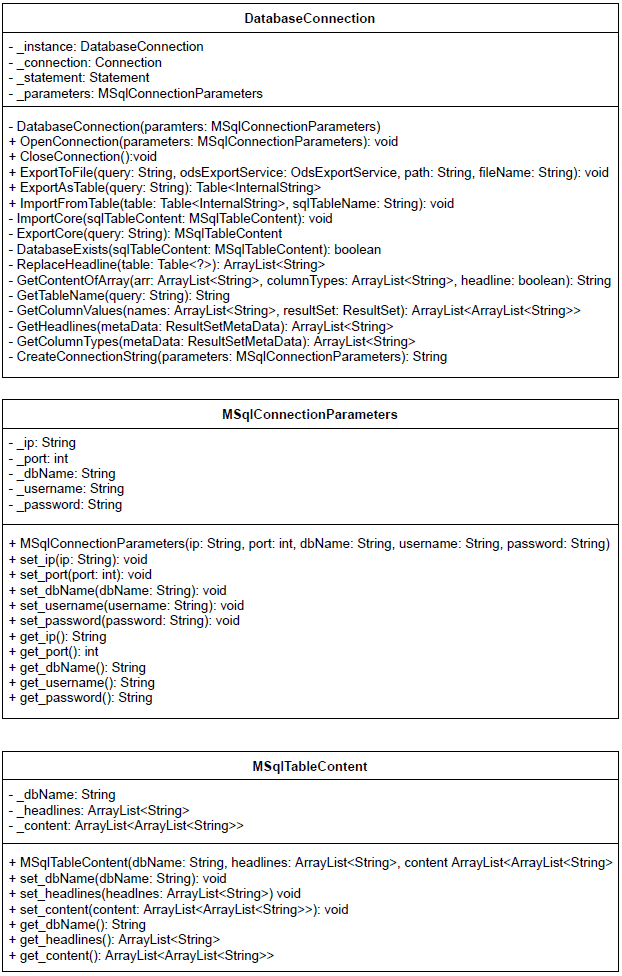
\includegraphics[width=0.75\textwidth]{images/mysql.png}
\caption{Klassendiagramm - MySQL}
\end{figure}

\subsection{Libre Office}
\label{subsectionLibreOffice}

\subsubsection{Kurzbeschreibung}
\label{loDescription}
Neben der internen Datenhaltung ist es wichtig eine Anbindung "nach außen" herzustellen. So soll es möglich sein, bis dato fremde Daten zusätzlich in die Statistik einbinden zu können. Hierzu wurde die Schnittstelle zu Libre Office Calc implementiert. Diese Anbindung ermöglicht es neben Daten, auch die dazugehörigen Tabellengestaltung beim Import auszulesen und abzuspeichern. Beim Export kann diese Operation durch definierte Funktionen in die andere Richtung durchgeführt werden. Doch dazu mehr im Kapitel \ref{loCore}.\\
Zunächst werden im folgenden die benötigten Objekte (Models) für das Arbeiten mit ods-Dateien vorgestellt.

\subsubsection{Models}
\label{loModels}

\textbf{MCell}\\
Dieses Model repräsentiert eine Zelle einer bestimmten Zeile und spalte. Dieses Objekt hat dabei einen "value" (Zelleninhalt) und Attribute, wie beispielsweise die Gestaltung der Zelle.

\begin{lstlisting}[caption=Repräsentation einer Zelle einer Libre Office Calc Datei, language=Java]
private HashMap<String,String> _attributes;
private Object _value;
\end{lstlisting}
\textbf{MColumn}\\
Eine Spalte einer Tabelle wird durch dieses Objekt widergespiegelt. Dabei kann eine Spalte nur Attribute wie die Gestaltung selbigen erhalten.
\begin{lstlisting}[caption=Repräsentation einer Spalte einer Libre Office Calc Datei, language=Java]
private HashMap<String,String> _attributes;
\end{lstlisting}
\textbf{MRow}\\
Neben den bekannten Attributen hält das repräsentierende Model für einer Zeile als zweite Property eine ArrayList von MCells.
\begin{lstlisting}[caption=Repräsentation einer Zeile einer Libre Office Calc Datei, language=Java]
private HashMap<String,String> _attributes;
private ArrayList<MCell> _cells;
\end{lstlisting}
\textbf{MTableWrapper}\\
Die gesamte Libre Office Tabelle kann mit Hilfe dieses Models dargestellt werden. Dieses Objekt hält die bereits eingeführten Attribute, wie auch eine ArrayList von Zeilen und Spalten.
\begin{lstlisting}[caption=Repräsentation einer Tabelle einer Libre Office Calc Datei inkl. aller Zeilen und Spalten, language=Java]
private HashMap<String,String> _attributes;
private ArrayList<MColumn> _columns;
private ArrayList<MRow> _rows;
\end{lstlisting}
\textbf{MSpreadsheet}\\
Mit den gerade aufgeführten Models ist es möglich, eine Tabelle mit deren Zeilen, Spalten und Zellen als Objekt darzustellen. Libre Office Calc-Dateien arbeiten aber mit so genannten Spreadsheets. Hierzu wurde das Model MSpreadsheet eingeführt. Dieses dient als Wrapper und kann mehrere Tabellen und die dazugehörigen Gestaltungen aller Bereiche aufnehmen. Somit können n Tabellen in die ArrayList vom Typ MTableWrapper gehalten werden.

\begin{lstlisting}[caption=Repräsentation einer kompletten Libre Office Calc Datei, language=Java]
private ArrayList<HashMap<String, String>> _fontStyles;
private HashMap<String, HashMap<String, String>> _tableStyles;
private HashMap<String, HashMap<String, String>> _rowStyles;
private HashMap<String, HashMap<String, String>> _columnStyles;
private HashMap<String, HashMap<String, String>> _cellStyles;
private ArrayList<MTableWrapper> _tables;
\end{lstlisting}
\textbf{MStyle}\\
Dieses Objekt dient als Wrapper, um einen Style beim Export zu einem ods-Format einzulegen. Dieser erhält eine Property property vom Typ OdfStyleProperty und der dazugehörige Wert, beispielsweise könnte es die property "FontWeight" mit dem Wert "bold" sein. Somit lässt sich ein Text in fett schreiben.

\begin{lstlisting}[caption=Repräsentation eines Styles einer Libre Office Calc Datei, language=Java]
private OdfStyleProperty property;
private String value;
\end{lstlisting}

\subsubsection{Kernfunktionalitäten}
\label{loCore}
\textbf{OdsExportService}\\
Zunächst ist wichtig zu erwähnen, dass zu Beginn des Exportvorganges zunächst der Konstruktor aufzurufen ist, um alle nötigen Objekte und Listen auf den Standardwert zu setzen. Hierbei kann ein parameterloser Konstruktor, wie auch ein Konstruktor mit einem Übergabeparameter aufgerufen werden. Der Unterschied liegt dabei nur an der Namensgebung der späteren Tabelle. Wird der leere Konstruktor aufgerufen, erhält die Tabelle einen Defaultnamen von "Table1". Dieser Wert kann durch den weiter angebotenen Konstruktor modifiziert werden.\\
Weiter kann durch zwei verschiedene Exporte gewählt werden. Zum einen ist es möglich, einen sofortigen Export einer MySQL-Datenbank in eine ods-Datei durch die Methode \textbf{InstantlyExportToFile} durchzuführen. Hierbei wird die Tabelle 1:1 in eine Libre Office Calc-Datei umgewandelt und es kann nichts modifiziert werden. Um eine komplett eigene Tabelle zu exportieren, kann \textbf{Export} aufgerufen werden. Diese Methode erhält als Übergabeparameter ein Table-Objekt mit allen Inhalten und Strukturen, als auch den Speicherort und den späteren Dateinamen.\\
Um eine ods-Datei korrekt zu exportieren, sind dabei folgende Schritte zu beachten:
\begin{enumerate} 
\item Tabelle erstellen - durch den Konstruktor oder \textbf{CreateTable(tableName: String): void})
\item Durch die Methode \textbf{AddHeadlines(headlines: ArrayList<String): void} kann die Tabelle Spaltenüberschriften versehen werden.
\item \textbf{AddContent(content: ArrayList<ArrayList<String{>}{>}): void} lässt es zu, neben den Überschriften, die dazugehörigen Daten einzupflegen.
\item Falls erwünscht: Style erstellen durch \textbf{CreateStyle(): void}
\item Nun ist es möglich, eine von den folgenden Eigenschaften hinzuzufügen
\begin{enumerate}
\item \textbf{SetBold(): void}
\item \textbf{SetItalic(): void}
\item \textbf{SetUnderline(): void}
\item \textbf{SetFontFamily(value: String): void}
\item \textbf{SetFontColor(value: String): void}
\item \textbf{SetFontSize(value: double): void}
\item \textbf{SetColumnWidth(columnIndex: int, value: double): void}
\item \textbf{SetRowHeight(rowIndex: int, value: double): void}
\item \textbf{SetTextAlign(value: String)}
\item \textbf{SetBackgroundColor(value: String) : void}
\end{enumerate}
\item Sind nun alle Eigenschaften für einen Style hinzugefügt worden, kann entschieden werden, welcher Bereich der Tabelle diesen Style bekommt. Dies ist möglich, indem eine der folgenden drei Methoden aufgerufen wird
\begin{enumerate}
\item \textbf{SetStyleToColumn(columnIndex: int): void}
\item \textbf{SetStyleToCell(rowIndex: int, columnIndex: int): void}
\item \textbf{SetStyleToRow(rowIndex: int): void}
\end{enumerate}
\end{enumerate}
\textit{Anmerkung: Die Schritte 4 bis 6 können nun beliebig oft aufgerufen werden. Möchte man beispielsweise drei Zeilen mit einem Style versehen, werden die Schritte folgedessen dreimal durchlaufen und abschließend dreimal die Methode \textbf{SetStyleToRow(rowIndex: int)} aufgerufen.}
\begin{lstlisting}[caption=Codebeispiel wie drei Zeilen einer Tabelle gestyled werden und eine weitere Tabelle hinzugefügt wird, language=Java]
var odsExportService = new OdsExportService("Table Number 1");
// ADD DATA TO TABLE
odsExportService.CreateStyle();
odsExportService.SetFontColor("#eaeaea");
odsExportService.SetStyleToRow(0);
// -------------------------------------------------------------
odsExportService.CreateStyle();
odsExportService.SetBackgroundColor("#ff0000");
odsExportService.SetStyleToRow(1);
// -------------------------------------------------------------
odsExportService.CreateStyle();
odsExportService.SetTextAlign("center");
odsExportService.SetStyleToRow(2);
// -------------------------------------------------------------
odsExportService.CreateTable("Table Number 2");
// ADD DATA TO TABLE
// -------------------------------------------------------------
odsExportService.SaveFile("C:/", "testTable");
\end{lstlisting}
Als letzte öffentliche Methode kann \textbf{SaveFile} angewendet werden, um mit Hilfe der Parameter "path" und "fileName" die generierte Tabelle in das ods-Dateiformat abzuspeichern. Hierbei wird das interne Spreadsheet-Objekt, das alle Styles, Strukturen und Inhalte enthält, an den angegebenen Speicherort exportiert.\\\\
\textbf{OdsImportService}\\
Der Import einer ods-Datei kann in zwei Varianten erfolgen. Zum einen ist es möglich, die eingelesen Daten mit \textbf{Import} anhand des übergebenen Pfades einzulesen. Der Rückgabewert dieser Funktion wäre ein Objekt vom Typ MSpreadsheet einzulesen. Die zweite Variante erfolgt auf die gleiche Art und Weise. Der Rückgabewert von \textbf{ImportFile} ist dabei ein mit dem InternalString typisiertes Objekt Table.

\subsubsection{Hilfsfunktionen}
\label{loHelper}
\textbf{OdsExportService}\\
Die in dieser Klasse verwendeten Hilfsmethoden unterstützen den Prozess beim Export zu einer ods-Datei. \textbf{AddContentFromTable} erzeugen die richtige Struktur den finalen Datei. Sie ist dafür zuständig, dass die Spalten bzw. die Zeilen und die darin liegenden Zellen das korrekte Format haben. Durch \textbf{CreateOdfStyle} wird ein neuer Style erstellt, der auf eine Tabellenzelle angewendet wird.\\
Um den Export von einem Table-Objekt durchzuführen, wurden die drei Hilfsmethoden \textbf{SetRowStylesFromTable}, \textbf{SetColumnStylesFromTable} und \textbf{SetCellStylesFromTable} eingeführt, um die Styles aus dem übergebenen Table-Objekt für die einzelnen Bereiche zu erhalten. Zur richtigen Selektierung des Styles wurde die Methode \textbf{WrapperSetStyleToTable} eingeführt, um anhand von einem bestimmten Keywort (z.B. font-color) die korrekte Stylemethode aufzurufen.
\textbf{OdsImportService}\\
Hauptaufgaben der implementierten privaten Methoden sind es, den erhaltenen XML-String, der ein Spreadsheet einer ods-Datei darstellt, den String in seine einzelnen Bestandteile bzw. Rubriken aufzuspliten. Dabei wird Rubrik und Styles, Tabellen, Zeilen, Spalten und Zellen verstanden. Die Methode \textbf{FindElementInXml} ruft dabei die restlichen Hilfsmethoden nacheinander auf. \textbf{CreateTableWrapper} und \textbf{\textbf{CreateAllLists}} generieren dabei alle benötigten Listen und starten das Suchen der einzelnen XML-Knoten.\\
Durch Knoten werden mit Hilfe von \textbf{VisitColumns} und \textbf{VisitRows} besucht und in das Wrapper-Objekt MTableWrapper eingefügt. In diesem Zuge werden die Styles vom eigentlichen Inhalt separat gehalten und auch separat in das MSpreadsheet-Objekt hinzugefügt. Die Styles werden durch die Methoden \textbf{FontStyles} und \textbf{StylesWrapper} aus dem XML-String selektiert.\\
Die nicht erklärten Methoden \textbf{GetNodeList}, \textbf{GetAttributes} und \textbf{SearchCell} wurden eingeführt, um die Iteration durch die XML-Struktur zu erleichtern.

\newpage
\subsubsection{Zusammenfassendes Klassendiagramm}
\label{loClasses}
\begin{figure}[h]
\centering
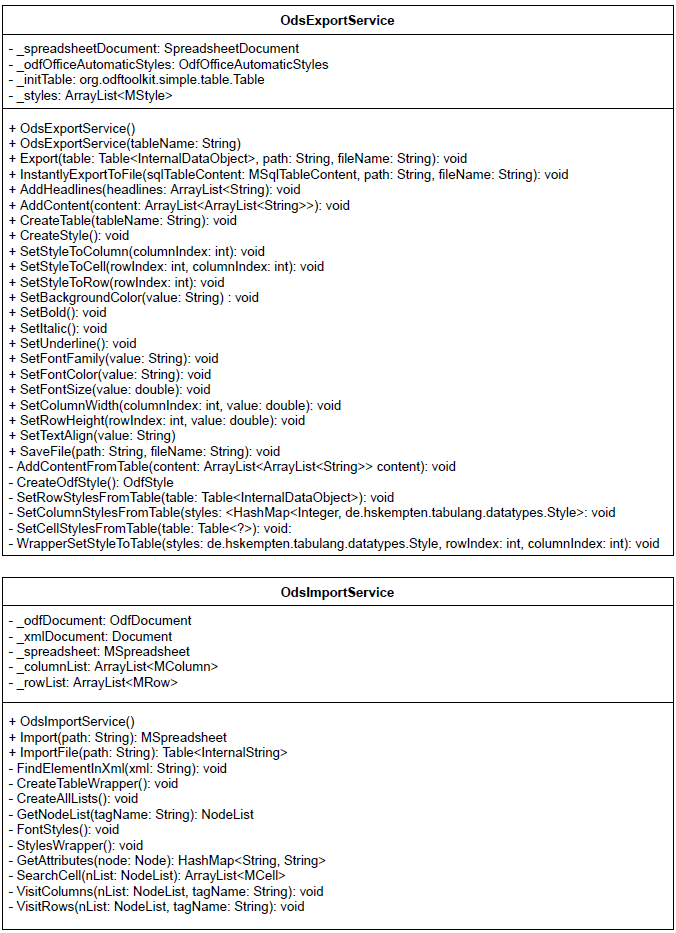
\includegraphics[width=0.75\textwidth]{images/ods.png}
\caption{Klassendiagramm - Libre Office Export und Import}
\end{figure}
\newpage
\begin{figure}[h]
\centering
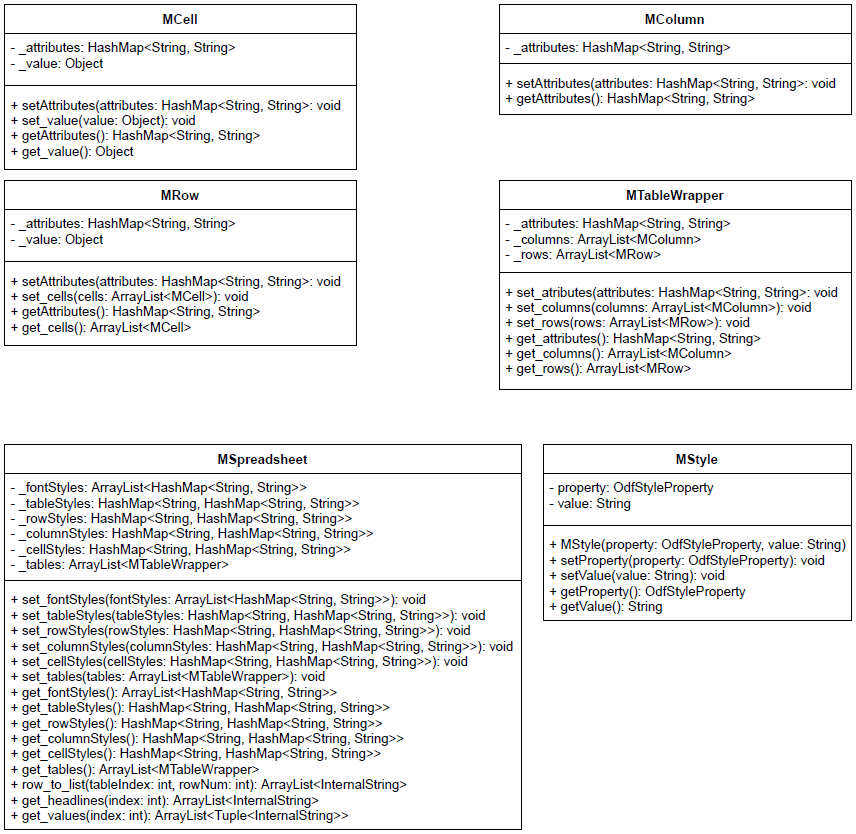
\includegraphics[width=0.75\textwidth]{images/ods-models.png}
\caption{Klassendiagramm - Libre Office Models}
\end{figure}